% !TEX TS-program = pdflatex
% !TEX encoding = UTF-8 Unicode

% This file is a template using the "beamer" package to create slides for a talk or presentation
% - Giving a talk on some subject.
% - The talk is between 15min and 45min long.
% - Style is ornate.

% MODIFIED by Jonathan Kew, 2008-07-06
% The header comments and encoding in this file were modified for inclusion with TeXworks.
% The content is otherwise unchanged from the original distributed with the beamer package.

\documentclass{beamer}


% Copyright 2004 by Till Tantau <tantau@users.sourceforge.net>.
%
% In principle, this file can be redistributed and/or modified under
% the terms of the GNU Public License, version 2.
%
% However, this file is supposed to be a template to be modified
% for your own needs. For this reason, if you use this file as a
% template and not specifically distribute it as part of a another
% package/program, I grant the extra permission to freely copy and
% modify this file as you see fit and even to delete this copyright
% notice. 


\mode<presentation>
{
  \usetheme{Berkeley}
  % or ...

  \setbeamercovered{transparent}
  % or whatever (possibly just delete it)
}

\usepackage{tikz}
\usepackage{graphicx}
\graphicspath{{C:/Users/garret/GoogleDrive/CEGA/CEGA-Programs/BITSS/Supporting-Material-Slides/APHRC/Images/}}
\usepackage[english]{babel}
% or whatever

\usepackage[utf8]{inputenc}
% or whatever

\usepackage{times}
\usepackage[T1]{fontenc}
% Or whatever. Note that the encoding and the font should match. If T1
% does not look nice, try deleting the line with the fontenc.


\title[Software and Workflow] % (optional, use only with long paper titles)
{Software and Workflow for Reproducible Research}

%\subtitle{Discussion} % (optional)

\author[Christensen] % (optional, use only with lots of authors)
{Garret Christensen\inst{1}}
% - Use the \inst{?} command only if the authors have different
%   affiliation.

\institute[UC Berkeley, Berkeley Initiatiative for Transparency in the Social Sciences] % (optional, but mostly needed)
{
  \inst{1}%
  UC Berkeley: Berkeley Initiative for Transparency in the Social Sciences\\
  Berkeley Institute for Data Science
}
% - Use the \inst command only if there are several affiliations.
% - Keep it simple, no one is interested in your street address.

\date[Short Occasion] % (optional)
{APHRC, Summer 2015}

\subject{Talks}
% This is only inserted into the PDF information catalog. Can be left
% out. 

\pgfdeclareimage[height=2cm]{university-logo}{C:/Users/garret/GoogleDrive/CEGA/CEGA-Programs/BITSS/Supporting-Material-Slides/APHRC/Images/BITSSlogo.png}
\logo{\pgfuseimage{university-logo}}

% Delete this, if you do not want the table of contents to pop up at
% the beginning of each subsection:
%\AtBeginSubsection[]
%{
%  \begin{frame}<beamer>{Outline}
%   \tableofcontents[currentsection,currentsubsection]
%  \end{frame}
%}


% If you wish to uncover everything in a step-wise fashion, uncomment
% the following command: 

\beamerdefaultoverlayspecification{<.->}

\begin{document}

% Since this a solution template for a generic talk, very little can
% be said about how it should be structured. However, the talk length
% of between 15min and 45min and the theme suggest that you stick to
% the following rules:  

% - Exactly two or three sections (other than the summary).
% - At *most* three subsections per section.
% - Talk about 30s to 2min per frame. So there should be between about
%   15 and 30 frames, all told.

\begin{frame}
  \titlepage
\end{frame}

\begin{frame}{Outline}
  \tableofcontents
  % You might wish to add the option [pausesections]
\end{frame}

\section{Introduction}

\begin{frame}{Reproducibility \& Transparency}
\begin{itemize}
\item What are problems associated with reproducibility?
\item What are solutions to these problems?
\item \textbf{What are practical tools to implement these solutions?}
\end{itemize}
\end{frame}
%%%%%%%%%%%%%%%%%%%%%%%%%%%%%%%%%%%%%%%%%%%%%%%%%%%%%%%%%%%%%%%%%%
\section{Problems}
\begin{frame}{Problems}
 \begin{itemize}
 \item Publication bias (see previous talk)
 \item Specification Searching (see previous talk)
 \item Data not available
 \item Code not available/unintelligible
 \item Code and data cannot reproduce original results
 \end{itemize}
\end{frame}

 
\subsection{Irreproducible Workflow}
 \begin{frame}{Irreproducible Workflow}
 \begin{itemize}
 \item
  Even with the original authors' help, you can't get the data to reproduce the published results. Or you just can't find the data to begin with. 
  \item \textit{Journal of Money, Credit, and Banking} Project. \href{http://www.jstor.org/stable/1806061}{(Dewald et al., AER 1986)}
   \item Martin Feldstein on Social Security and private savings, Reinhart and Rogoff on debt and GDP growth.
 \end{itemize} 
 \end{frame}
%%%%%%%%%%%%%%%%%%%%%%%%%%%%%%%%%%%%%%%%%%%%%%%%%%%%%%%%%%%%%%%%%%%%

\section{Solutions}
\begin{frame}{Solutions}
\begin{itemize}[<+->]
\item Study Registry (see previous talk)
\item Pre-Analysis Plan (see previous talk)
\item Reproducible Workflow
\end{itemize}
\end{frame}

%%%%%%%%%%%%%%%%%%%%%%%%%%%%%%%%%%%%%%%%%%%%%%%%%%%%%%%%%%%%%%%%%%%%%

\subsection{Workflow}
\begin{frame}{Reproducible Workflow}
 \begin{itemize}
 \item Literate Programing 
 \item Version control with \href{http://www.github.com}{Github} or \href{http://osf.io}{OSF}.
  \item R Markdown and \href{http://rstudio.com}{R Studio} to write dynamic documents.
 \item Data Sharing
 \begin{itemize}
 \item \href{http://www.thedata.org}{Harvard's Dataverse}
 \end{itemize}
\end{itemize}
\end{frame}
%%%%%%%%%%%%%%%%%%%%%%%%%%%%%%%%%%%%%%%%%%%%%%%%%%%%%%%%%%%%%%%%%%%%%
\subsection{Literate Programming}
\begin{frame}{Literate Programming}
\begin{itemize}
\item First, \textit{programming} is key to reproducibility. Working in Excel is not reproducible.
\item See Reinhart and Rogoff ``Growth in a Time of Debt'' controversy: 
\begin{itemize}
	\item
	Original Paper, \href{https://www.aeaweb.org/articles.php?doi=10.1257/aer.100.2.573}{\textit{AER P \& P} 2010}
	\item 
	\href{http://cje.oxfordjournals.org/content/38/2/257}{Herndon et. al (2013)} finding.
	\item \href{http://www.newyorker.com/news/john-cassidy/the-reinhart-and-rogoff-controversy-a-summing-up}{\textit{New Yorker} summary}.
\end{itemize}

\item Random number generation in Excel: set seed with \href{http://www.statisticshowto.com/use-random-number-generator-excel/}{Data Analysis Toolpak}. 
\end{itemize}
\end{frame}

\begin{frame}{Literate Programming}
\begin{itemize}
\item  If you are using SPSS, use of `syntax' to record all the commands you run is simple. (See \href{http://www.ats.ucla.edu/stat/spss/seminars/spss_syntax/}{UCLA tutorial}.) Similarly in Stata, `commandlog'.

\item Better is to write scripts. R, Stata, SAS, Python, or whatever you please.

\item Open source has some advantages (being free, for one) but you're going to use what everyone in your field uses.
\end{itemize}
\end{frame}

\begin{frame}{Literate Programming}
\begin{itemize}
\item
Second, \textit{literate programming} is key to reproducibility. Write code to be read by a human being, with the code for the computer secondary.
\end{itemize}
\end{frame}

\begin{frame}{Literate Programming}
\begin{quote}
``I believe that the time is ripe for significantly better documentation of programs, and that we can best achieve this by considering programs to be works of literature. Hence, my title: ``Literate Programming.''

Let us change our traditional attitude to the construction of programs: Instead of imagining that our main task is to instruct a computer what to do, let us concentrate rather on explaining to human beings what we want a computer to do.
\end{quote}
(cont.)
\end{frame}

\begin{frame}{Literate Programming}
\begin{quote}
``The practitioner of literate programming can be regarded as an essayist, whose main concern is with exposition and excellence of style. Such an author, with thesaurus in hand, chooses the names of variables carefully and explains what each variable means. He or she strives for a program that is comprehensible because its concepts have been introduced in an order that is best for human understanding, using a mixture of formal and informal methods that reinforce each other.''
\end{quote}
--Donald Knuth \textit{The Computer Journal}, 1984
\href{http://www.literateprogramming.com/index.html}{\beamerbutton{Quotes}}
\href{http://comjnl.oxfordjournals.org/content/27/2/97.full.pdf+html}{\beamerbutton{Original}}
\end{frame}

\subsection{Workflow Suggestions}
\begin{frame}{Organizing and Recording Workflow}
\begin{quote}
``Reproducibility is just collaboration with people you don't know,
including yourself next week''
\end{quote}
\begin{flushright}
---Philip Stark, UC Berkeley Statistics
\end{flushright}
\end{frame}

\begin{frame}{Organizing and Recording Workflow}
 Practical coding and organizational suggestions
 \begin{itemize}
 \item Long (2008) \textit{The Workflow of Data Analysis Using Stata}
 \item Making any changes to a file that has been posted/shared means it gets a new name.
 \item Use version commands to ensure others get same results.
 \item Keep a daily research log.
 \item Take the tiem 
\end{itemize}
\end{frame}
%%%%%%%%%%%%%%%%%%%%%%%%%%%%%%%%%%%%%%%%%%%%%%%%%%%%%%%%%%%%%%%%%%%%%
\subsection{Version Control}
\begin{frame}{Version Control}
\begin{itemize}[<+->]
\item
Using version control (AKA revision control) can help to make your work more reproducible.

\item
What is version control?

\begin{quote}
Version control is a system that records changes to a file or set of files over time so that you can recall specific versions later. For the examples in this book you will use software source code as the files being version controlled, though in reality you can do this with nearly any type of file on a computer.
\end{quote}
--Git, \href{https://git-scm.com/book/en/v2/Getting-Started-About-Version-Control}{About Version Control}

%\item Distributed Version Control Systems (DCVS) let multiple users control the same files in this manner.
\end{itemize}
\end{frame}
%%%%%%%%%%%%%%%%%%%%%%%%%%%%%%%%%%%%%%%%%%%%%%%%%%%%%%%
\begin{frame}{Version Control}
With version control you can:
\begin{itemize}
\item Collaborate 
\item Track who made every change
\item Easily switch between versions of files
\item Compare versions of files
\item Backup
\item Work with the same files on different machines
\item Experiment with a new version of code without breaking things
\end{itemize}
\href{http://stackoverflow.com/questions/1408450/why-should-i-use-version-control}{\beamerbutton{Link1}}
\href{http://tex.stackexchange.com/questions/1118/what-are-the-advantages-of-using-version-control-git-cvs-etc-in-latex-documen}{\beamerbutton{Link2}}
\href{http://stackoverflow.com/questions/1408450/why-should-i-use-version-control}{\beamerbutton{Link3}}
\end{frame}
%%%%%%%%%%%%%%%%%%%%%%%%%%%%%%%%%%%%%%%%%%%

\begin{frame}{Version Control}
Places you're already using version control without knowing it:
\end{frame}
%%%%%%%%%%%%%%%%%%%%%%%%%%%%%%%%%%%%%%%


{ % all template changes are local to this group.
    \setbeamertemplate{navigation symbols}{}
    \begin{frame}[plain]
        \begin{tikzpicture}[remember picture,overlay]
            \node[at=(current page.center)] {
                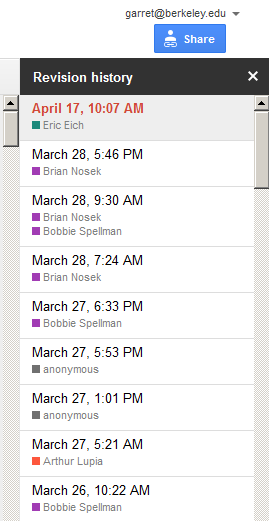
\includegraphics[height=\paperheight]{googledocs.PNG}
            };
        \end{tikzpicture}
     \end{frame}

 \setbeamertemplate{navigation symbols}{}
    \begin{frame}[plain]
        \begin{tikzpicture}[remember picture,overlay]
            \node[at=(current page.center)] {
                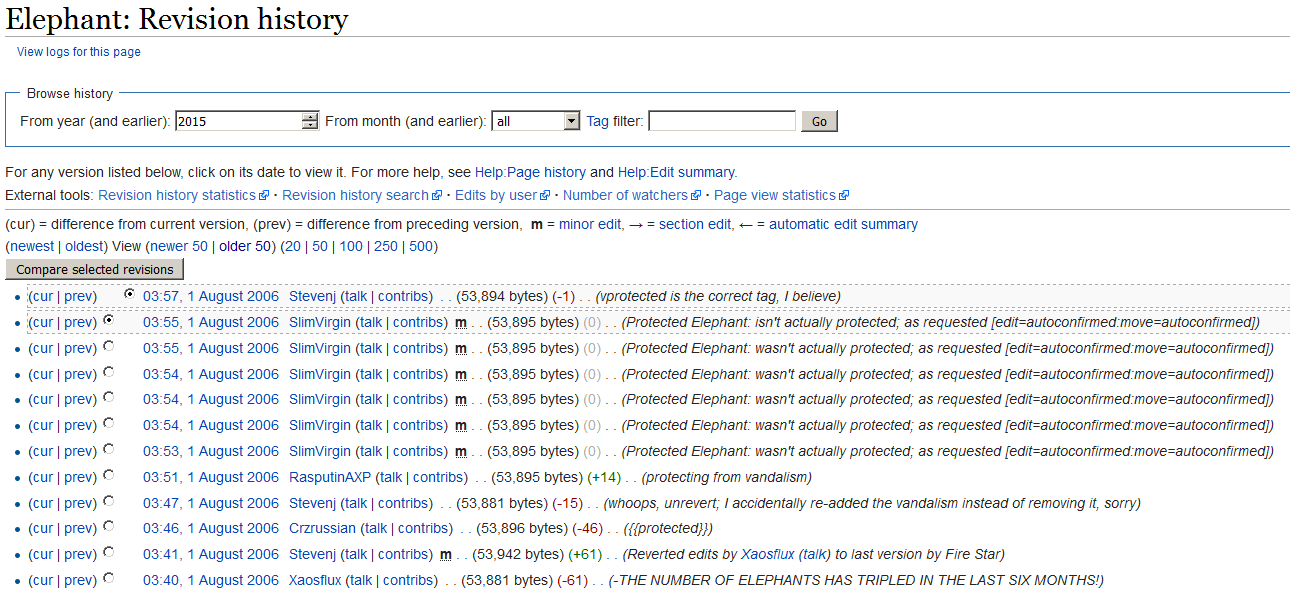
\includegraphics[width=\paperwidth]{elephantswiki.PNG}
            };
        \end{tikzpicture}
     \end{frame}
}
\begin{frame}{Version Control}
Places you're already using version control without knowing it:
\begin{itemize}
	\item
	Google Docs
	\item
	Wikipedia
	\item
	Every piece of software you use.
\end{itemize}
\end{frame}

%%%%%%%%%%%%%%%%%%%%%%%%
\begin{frame}{Version Control}
Isn't this just a complicated version of the ``date and initial'' method?
\begin{itemize}
\item regressions2015.08.24.do
\item regressions2015.08.25.do
\item regressions2015.08.25GC.do
\item Hassle
\item Confusion
\end{itemize}
\end{frame}

\begin{frame}{Version Control}
\begin{quote}Here is a good rule of thumb: If you are trying to solve a problem, and there are multi-billion dollar  firms  whose  entire  business  model  depends  on  solving  the  same  problem,  and  there  are whole courses at your university devoted to how to solve that problem, you might want to figure out what the experts do and see if you can’t learn something from it.

...

Not one piece of commercial software you have on your PC, your phone, your tablet,
your car, or any other modern computing device was written with the “date and initial” method.
\end{quote}
--Matthew Gentzkow and Jesse M. Shapiro ``\href{http://web.stanford.edu/~gentzkow/research/CodeAndData.pdf}{Code and Data for the Social Sciences: A Practitioner's Guide}''
\end{frame}


{ % all template changes are local to this group.
    \setbeamertemplate{navigation symbols}{}
    \begin{frame}[plain]
        \begin{tikzpicture}[remember picture,overlay]
            \node[at=(current page.center)] {
                
\includegraphics[height=\paperheight]{github-logo-transparent.jpg}
            };
        \end{tikzpicture}
     \end{frame}

    \begin{frame}[plain]
        \begin{tikzpicture}[remember picture,overlay]
            \node[at=(current page.center)] {
                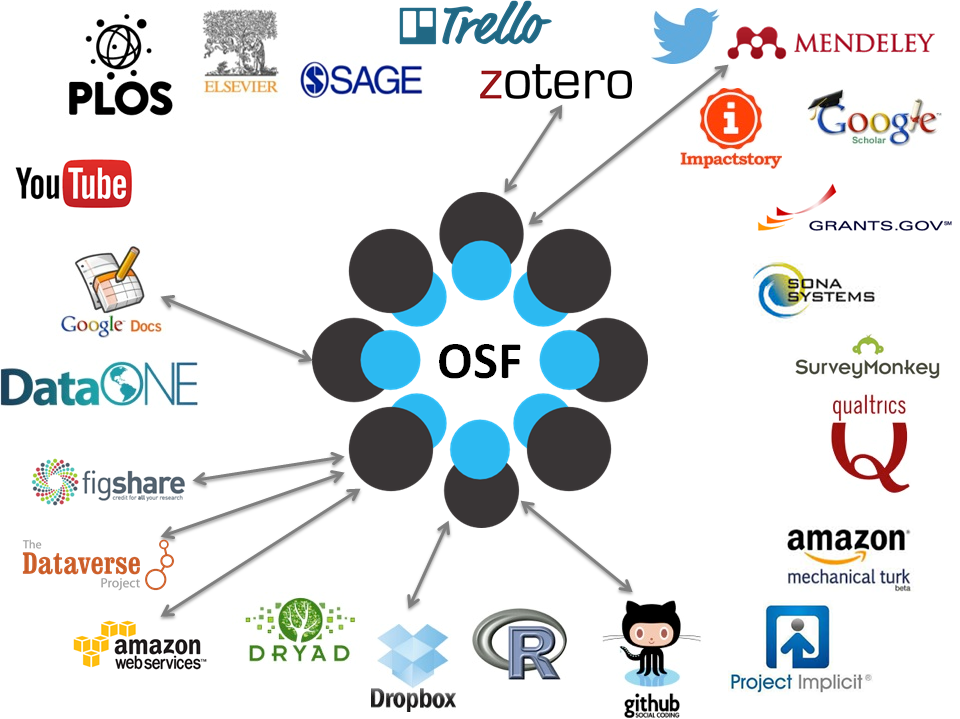
\includegraphics[height=\paperheight]{OSFnow.PNG}
            };
        \end{tikzpicture}
     \end{frame}
 
    \begin{frame}[plain]
        \begin{tikzpicture}[remember picture,overlay]
            \node[at=(current page.center)] {
                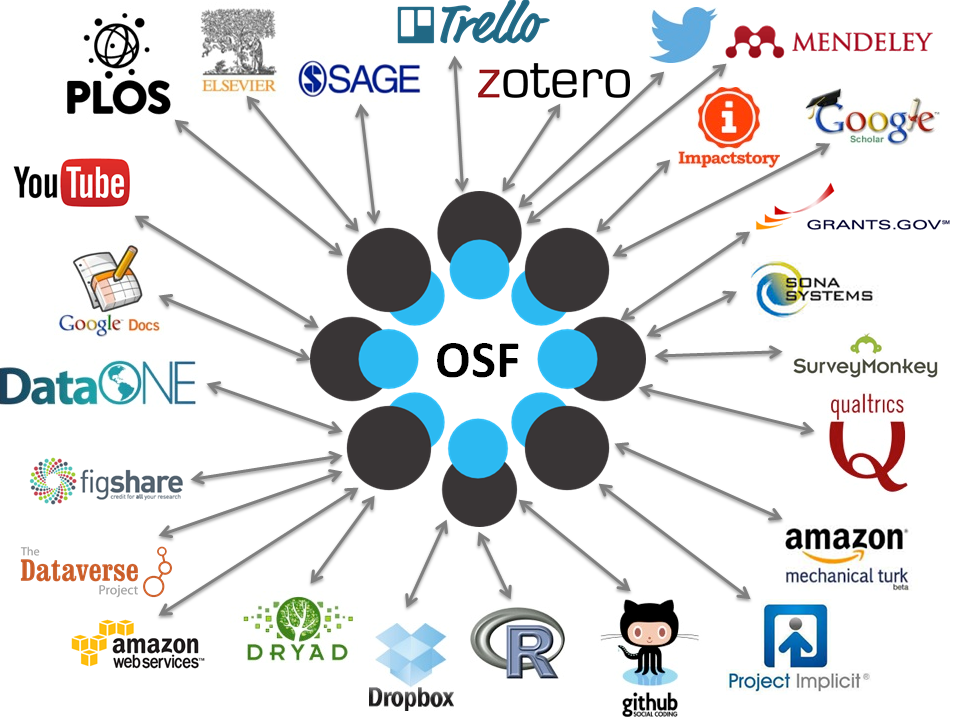
\includegraphics[height=\paperheight]{OSFsoon.PNG}
            };
        \end{tikzpicture}
     \end{frame}
}
%%%%%%%%%%%%%%%
\begin{frame}{Examples}
GitHub and OSF Examples:
\begin{itemize}
\item
Slides for this workshop on Github.com
\item \url{http://www.github.com/bitss/aphrc}
\item
Slides also available on the Open Science Framework
 \item \url{https://osf.io/m5ey4/}
\end{itemize}
\end{frame}
%%%%%%%%%%%%%%%%%%%%%%%%%%%%%%%%%%%%%%%%%%%%%%%%%%%%%%%%%%%%%%%%%%%%%
\subsection{Dynamic Documents}
\begin{frame}{Dynamic Documents}
\begin{itemize}[<+->]
\item
Even if you write perfect (version controlled) code, you can still run into problems going from your code to paper. This is where \textit{dynamic documents} come in.
\item
A dynamic document includes your data, code, analysis, and output all in one place. Fully automated, you can guarantee no mistakes from copying and pasting.
\item
Do this with \href{http://rmarkdown.rstudio.com/}{R Markdown} in \href{https://www.rstudio.com/}{R Studio} or 
\href{http://haghish.com/statistics/stata-blog/reproducible-research/ketchup.php}{Ketchup} in Stata.
\end{itemize}
\end{frame}


\begin{frame}{Dynamic Documents}
\begin{itemize}
\item Include tables by linking to a file, instead of a static image.
\item Include number by linking to a value calculated by an analysis file, instead of a static number typed manually.
\item Automatically update tables and numbers.
\item Produce entire paper with one or two clicks.
\end{itemize} 
\end{frame}


\begin{frame}{Examples}
\begin{itemize}
\item
R Studio Example
\item
Stata Example
\end{itemize}
\end{frame}
%%%%%%%%%%%%%%%%%%%%%%%%%%%%%%%%%%%%%%%%%%%%%%%%%%%%%%%%%%%%%%%%%%%%%
%\subsection{Data Sharing}
%\begin{frame}{Data Sharing}
%Make all your data and code publicly available.

%Put it in a place where people can find it. 

% For APHRC that might be the APHRC repository.
%\end{frame} 
%%%%%%%%%%%%%%%%%%%%%%%%%%%%%%%%%%%%%%%%%%%%%%%%%%%%%%%%%%%%%

\section{Conclusion}
\begin{frame}{Conclusion}
Simple tools exist to help you transparently and reproducibly take your research from beginning to end. 
\begin {itemize}
\item Trial Registries (previous slides)
\item Pre-Analysis Plans (previous slides)
\item Version Control
\item Open Science Framework
\item Dynamic Documents
\item Trusted Public Data Archive (next slides)
\end{itemize} 
\vspace{0.25in}
Read more in my \href{http://github.com/garretchristensen/manual}{\textit{Manual of Best Practices in Transparent Social Science Research}} on GitHub.
\end{frame}



\end{document}


